\begin{tikzfigure}
    \subcaptionbox{10th harmonic scattering.}{
        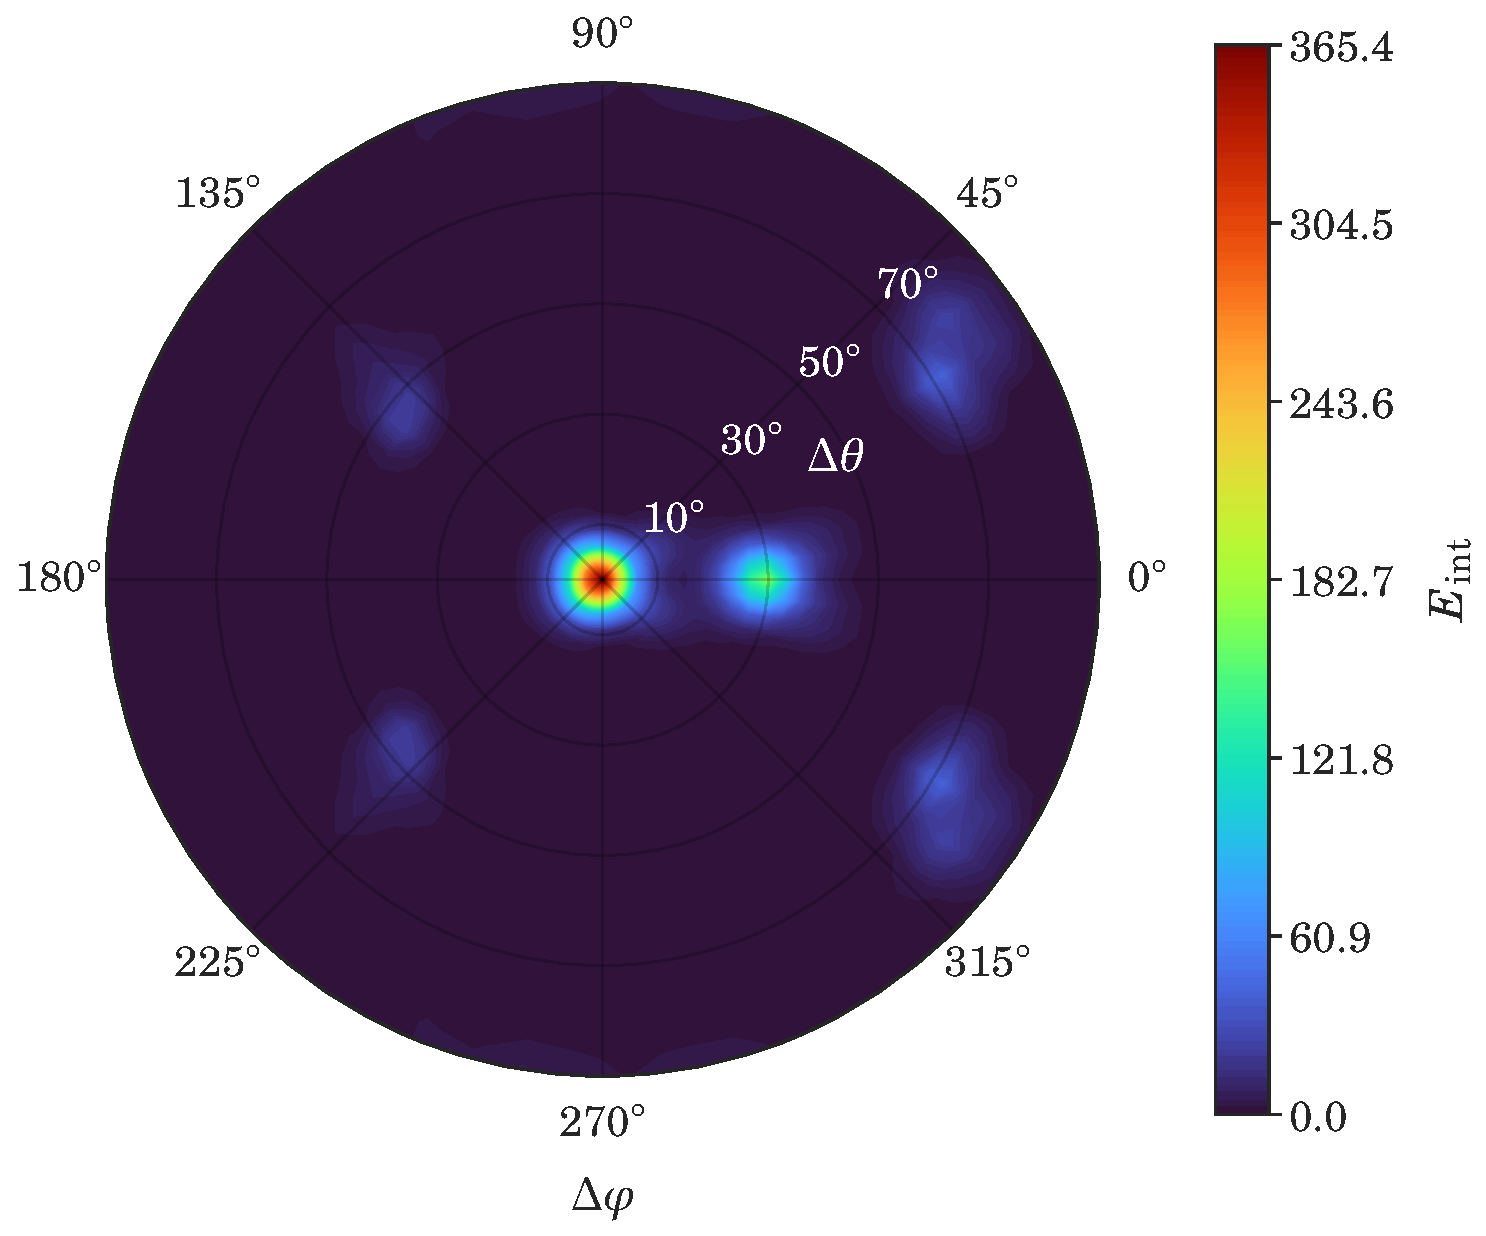
\includegraphics[width=0.48\linewidth]{../img/celes/E_squared/eint_10harm_15deg_0.0nonreg.pdf}
    }
    \hfil
    \subcaptionbox{Wavepacket scattering.}{
        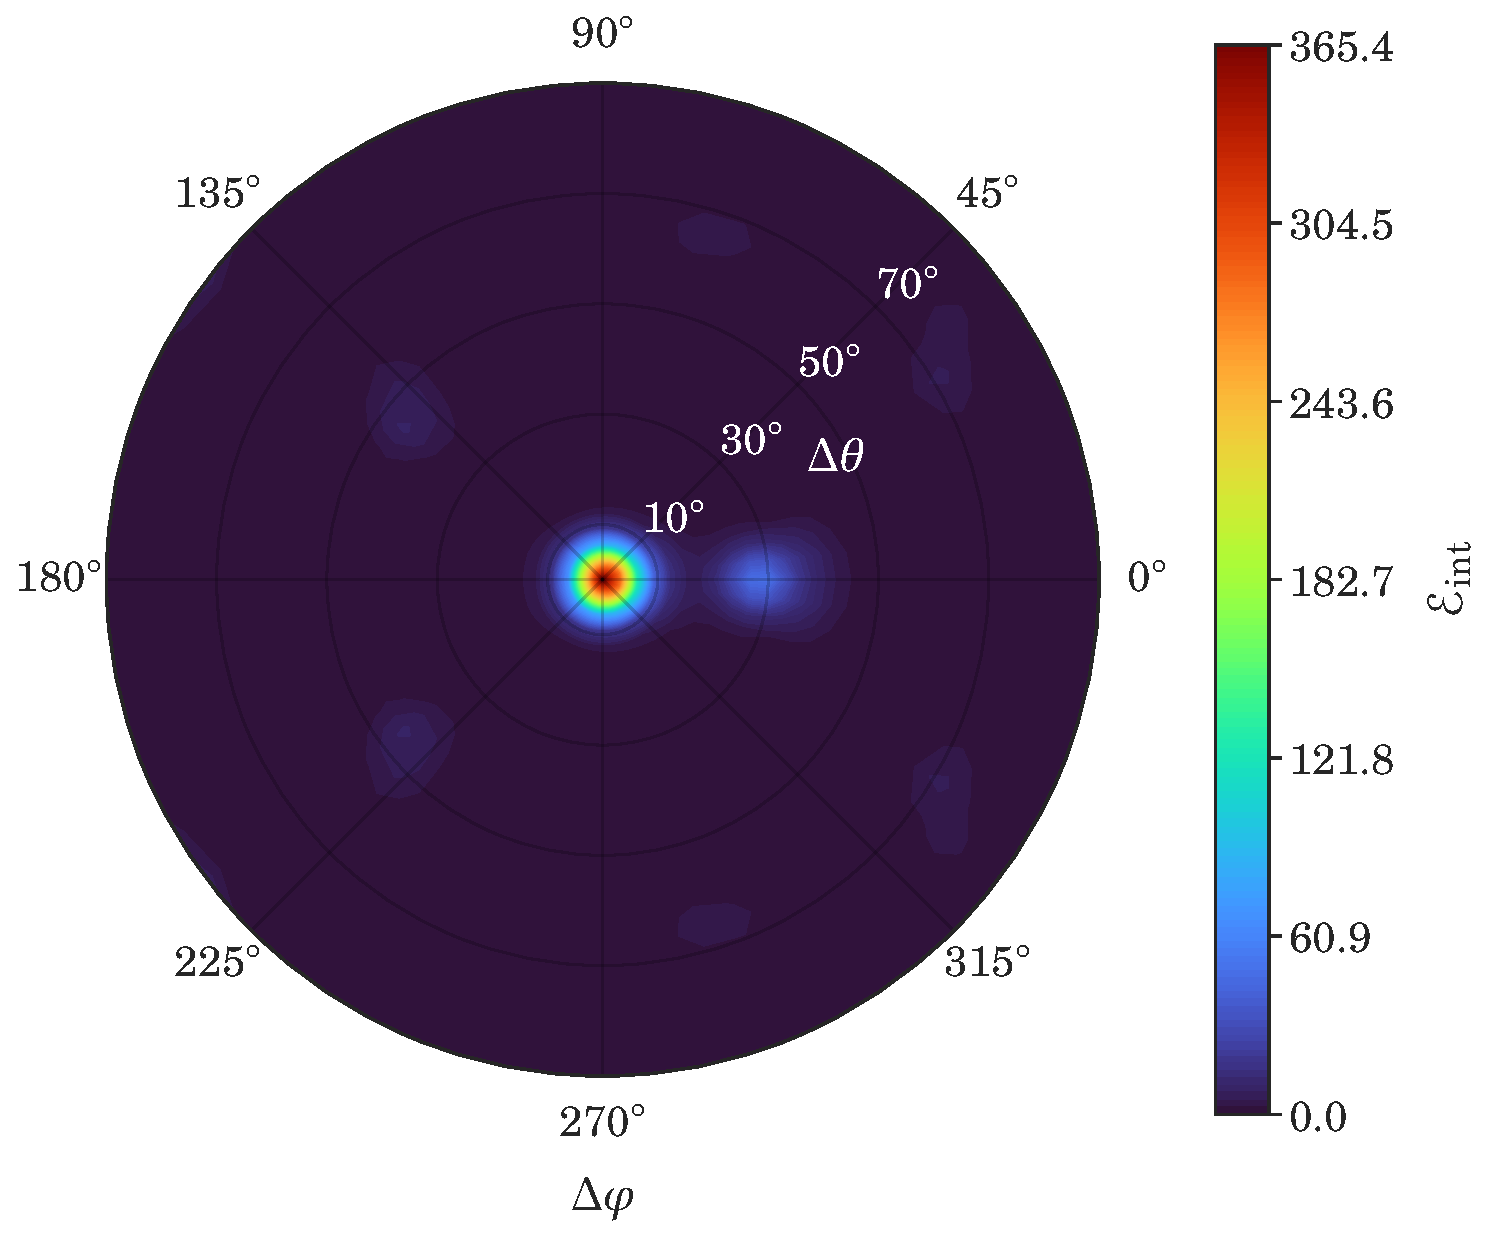
\includegraphics[width=0.48\linewidth]{../img/celes/E_squared/eint_wavepacket2_15deg_0.0nonreg.pdf}
    }
    \label{wavepacket1:image}\caption{Angular scattering diagram of a Gaussian wave packet and the 10th harmonic. $\theta_0 = 15^\circ$, $\varphi_0 = 0^\circ$, $d = 2\lambda_{10}$, cluster radius $a = 20$ nm.}
\end{tikzfigure}

\begin{tikzfigure}
    \subcaptionbox{Scattering by a single-row array of clusters.}{
        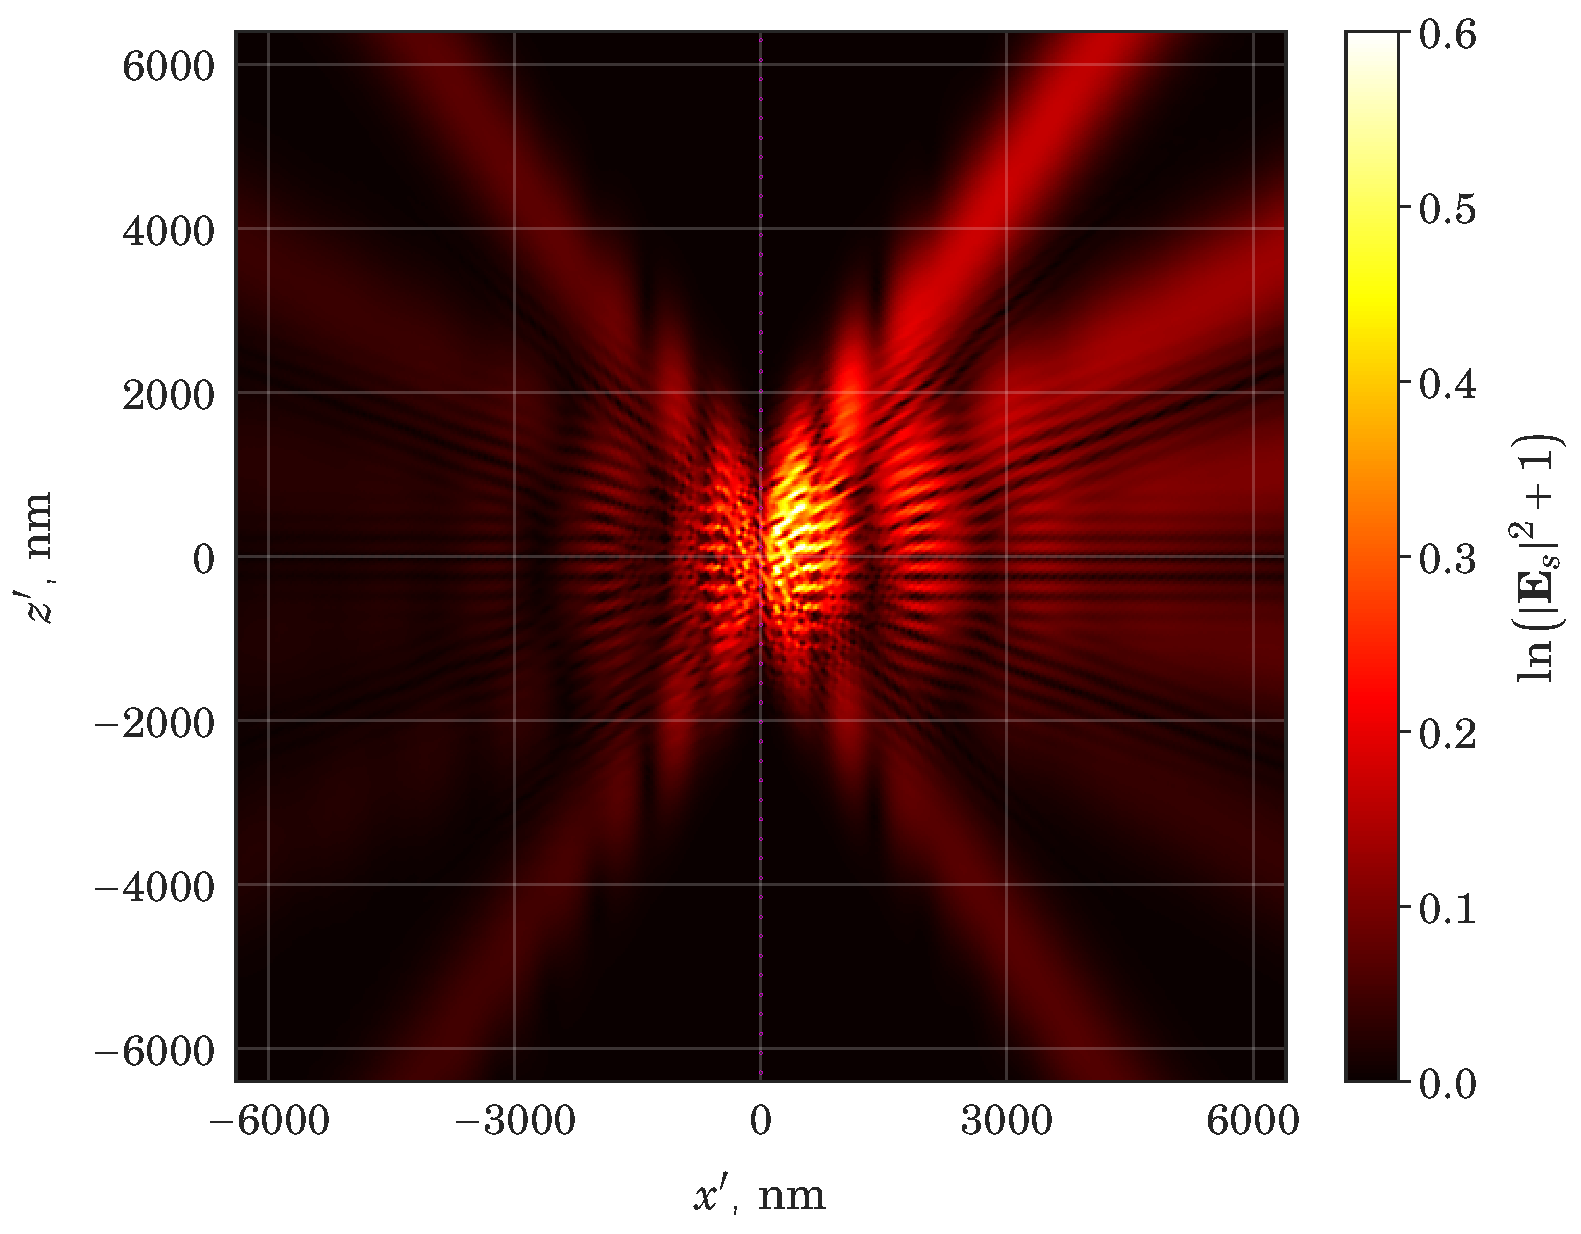
\includegraphics[width=0.48\linewidth]{../img/celes/plane_flat_to_compare.pdf}
    }
    \hfil
    \subcaptionbox{Scattering by a three-row array of clusters.}{
        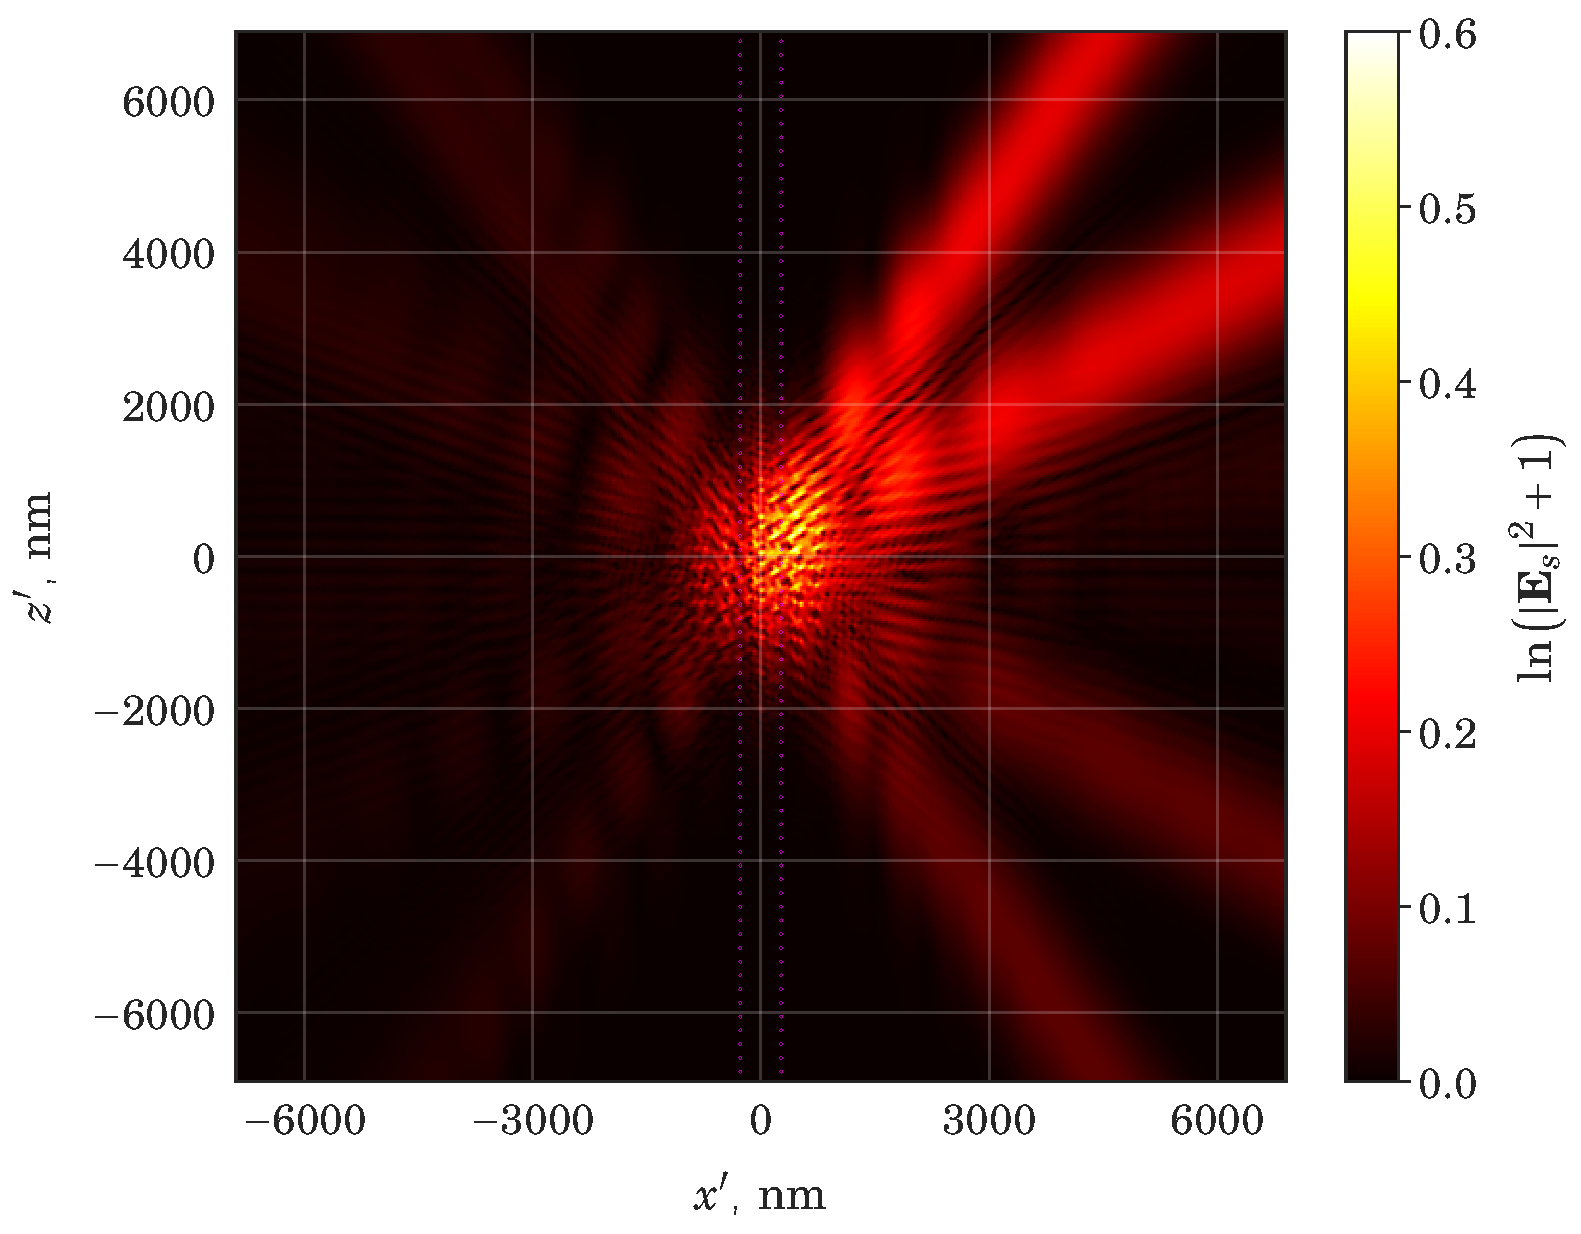
\includegraphics[width=0.48\linewidth]{../img/celes/3plane_flat_to_compare.pdf}
    }
    \label{cluster_rows:image}\caption{Scattering of a harmonic with $\lambda \approx 89$ nm by an array of clusters, $\varphi_0 = 0^\circ$, $\theta_0 = 30^\circ$, $a = 30$ nm, the distance between clusters is $d = 3\lambda$, the incident field is directed from the lower left corner to the upper right at an angle $\theta_0$ with respect to the normal to the target.}
\end{tikzfigure}